\documentclass[runningheads,a4paper]{llncs}
%
\usepackage{graphicx}

\setcounter{tocdepth}{3}

\usepackage[usenames]{color}
\usepackage[usenames,dvipsnames]{xcolor}
\usepackage{listings} \usepackage{color}
\usepackage{textcomp} % needed for 'upquote' option below
\definecolor{ListingColor}{RGB}{248,248,248}
\lstset{ %
  %language=Ruby,                % the language of the code
  upquote=true,                 % use straight quotes not curly quotes
  basicstyle=\scriptsize\ttfamily\upshape,       % the size and style of the fonts that are used for the code
  commentstyle=\slshape,
  xrightmargin=0.1in,
  xleftmargin=0.2in,
  numbers=none,                   % where to put the line-numbers
  numberstyle=\footnotesize,      % the size of the fonts that are used for the line-numbers
  stepnumber=1,                   % the step between two line-numbers. If it's 1, each line 
  % will be numbered
  numbersep=8pt,                  % how far the line-numbers are from the code
  backgroundcolor=\color{ListingColor},  % choose the background color. You must add \usepackage{color}
  showspaces=false,               % show spaces adding particular underscores
  showstringspaces=false,         % underline spaces within strings
  showtabs=false,                 % show tabs within strings adding particular underscores
  frame=trbl,                   % adds a frame around the code
  tabsize=2,                      % sets default tabsize to 2 spaces
  captionpos=b,                   % sets the caption-position to bottom
  breaklines=true,                % sets automatic line breaking
  breakatwhitespace=false,        % sets if automatic breaks should only happen at whitespace
  %title=\lstname,                 % show the filename of files included with \lstinputlisting;
  % also try caption instead of title
  escapeinside={\%*}{*)},         % if you want to add a comment within your code
  morekeywords={*,...}            % if you want to add more keywords to the set
}


\newcommand{\tbd}[1]{{\color{Red}\bf{TBD: #1}\normalfont}}

\newcommand{\uf}[1]{\footnote{\url{http://#1}}}

%
\begin{document}
\renewcommand{\keywords}[1]{\par\addvspace\baselineskip\noindent\keywordname\enspace\ignorespaces#1}
%
\mainmatter




\title{MAGIC: Massive Automated Grading in the Cloud}
% a short form should be given in case it is too long for the running head
\titlerunning{Massive Automated Grading in the Cloud}

\author{Armando Fox\inst{1} 
\and David Patterson\inst{1} 
\and Samuel Joseph\inst{2} 
\and Paul McCulloch\inst{3}}
\authorrunning{Armando Fox et al.}

\institute{University of California, Berkeley
\and Hawai'i Pacific University and AgileVentures
\and Apex Computing Inc. and AgileVentures}

\toctitle{Lecture Notes in Computer Science}
\tocauthor{}
\maketitle

\begin{abstract}

%% must be 70-150 words to meet LNCS guidelines

We describe our experience developing and using a specific category of
cloud-based autograder (automatic evaluator of student programming
assignments) for software engineering.  To
establish our position in the landscape, our autograder is \emph{fully
automatic}, rather than serving to increase instructor productivity
during manual grading, and \emph{test based}, in that 
it exercises student code under controlled conditions rather than
relying on static analysis or comparing only the output of student
programs against reference output.  We include a brief description of
the course for which 
the autograders were built, \emph{Engineering Software as a Service},
and the rationale for building them in the 
first place, since we had to surmount some new obstacles related to the
scale and delivery mechanism of the course.
In three years of using the autograders in conjunction with both a
software engineering MOOC and the residential course on which the MOOC
is based, they have reliably graded hundreds of thousands of student
assignments, and are currently being refactored to make their code more
easily extensible and maintainable.  We have found cloud-based
autograding to be scalable,
sandboxable, and reliable, and students value the near-instant feedback
and opportunities to resubmit homework assignments more than once.
Our open-source, cloud-based, producer-consumer
autograder architecture allows custom autograders to be plugged in
easily, and while it is currently compatible
with the OpenEdX platform, it should be easy to plug into other Learning
Management Systems.


\keywords{TBD keywords here} \tbd{need keywords}

\end{abstract}

\section{Background: Autograding for a Software Engineering Course}

Automated assessment of student programming assignments was first tried
over fifty years ago~\cite{hollingsworth60}, and with the arrival of
Massive Open Online Courses (MOOCs), so-called ``autograders'' are
receiving renewed attention.  The appeal is obvious: students not only
get immediate feedback, but can now be given multiple opportunities to
resubmit their code to improve on their mistakes, providing the
opportunity for mastery learning.  Over their long history, autograders
have evolved from test-harness libraries that must be linked against
student code to web-based systems that perform both dynamic tests and static
analysis~\cite{douce-2005-autograding-survey}.  Autograders have also
found use in residential classrooms, with some instructors even finding
that grades on autograded programming assignments are a surprisingly good
predictor of final course grades~\cite{navrat2014}.

\tbd{Transition needed}

From 2008 to 2010, authors Fox and Patterson refocused
UC~Berkeley's one-semester (14-week) undergraduate software engineering
course~\cite{crossing_the_software_chasm,agile_sw_curriculum} on agile
development, emphasizing
behavior-driven design (BDD)~\cite{bdd} and automated testing.  A key
 philosophy of the redesign
was that whenever we advised students to use a certain
methodology such as behavior-driven
development, we would provide them with a best-of-breed tool to immediately
practice that methodology.  These tools would not only enable the
students to learn immediately by doing, but also provide quantitative
feedback for instructors to check students' work.  
We chose Ruby on Rails as the teaching vehicle because its developer
ecosystem has by far the richest set of such tools, with a much stronger
emphasis on high productivity, refactoring, and beautiful code than any
other ecosystem we'd seen.
The choice of Rails in turn influenced our decision to use Software as a
Service (SaaS) as the learning vehicle, rather than (for example) mobile
or embedded apps.
Among the tools we
use~\footnote{All are either open source downloads or offer a free
hosted version sufficient for class projects.  Web
sites: \texttt{rspec.info}, \texttt{github.com/colszowka/simplecov}, \texttt{cukes.info}, \texttt{pivotaltracker.com}, \texttt{travis-ci.org}, \texttt{codeclimate.com}, \texttt{github.com}.} 
are 
RSpec for unit testing,
SimpleCov for C0 test coverage,
Cucumber for behavior-driven design and integration testing,
Pivotal Tracker for lightweight project management,
Travis for continuous-integration testing,
CodeClimate for code-quality metrics,
and, of course, GitHub, with which all the
other tools communicate.  
Thus, in just 14 weeks, third- and fourth-year students learn Ruby
and Rails (most haven't seen it before), learn the above tools, complete
five programming assignments, take three exams, and form ``two-pizza
teams'' of 4--6 to prototype a real SaaS application for a nonprofit,
NGO, or campus unit, over four two-week agile iterations.

The new course was offered experimentally in 2009--2010 and was
immediately successful; growing enrollment demand (from 45 in the pilot
to 240 in Spring 2015) led 
us to write a book around the course~\cite{esaaS} and to start thinking
about how to scale it up.  
Coincidentally, in mid-2011 our colleagues Prof.~Andrew Ng
and Prof.~Daphne Koller at Stanford were experimenting with a MOOC
platform which would eventually become Coursera, and invited us to try
adapting part of our course to the
platform as an experiment.  With the help of some very strong teaching
assistants, we not only created Berkeley's first MOOC, but also the
initial versions of the autograder technology described here.  To date,
we estimate over 1,500 engineer-hours have been invested in the
autograders, including contributions from MOOC alumni,
from the AgileVentures\uf{agileventures.org}  open development community,
and from
instructors using our MOOC materials as a SPOC~\cite{moocs-spocs-TR}.


\section{Cloud Grading Architecture With OpenEdX}
\label{sec:arch}

We adopt a narrow Unix-like view of an autograder: it is a
stateless command-line program that, given a student work submission and
a rubric, computes a score and some textual feedback.  We treat
separately the question of how to connect this program to an LMS.
All other policy issues---whether students can resubmit homeworks, how
late penalties are computed, where the gradebook is stored, and so 
on---are out of scope\footnote{Due to an implementation
  artifact of OpenEdX, the autograders currently do adjust their scores
  to reflect late penalties, based on metadata about due dates provided
  with each assignment submission.}, as is the question of whether these
autograders should replace or supplement manual grading by instructors.

\subsection{Why Another Autograder?}

Given that 17 autograding systems and over 60 papers about them were
produced from 2006--2010 alone~\cite{ihantola-2010-autograding-survey},
why did we choose to build our own?
First, as the survey authors point
out, many existing systems' code
is not readily available or is tightly integrated to a particular Learning
Management System (LMS).  We needed to integrate with Coursera and
later OpenEdX, both of which were new and had not yet embraced
standards such as Learning Tools Interoperability\uf{imsglobal.org/lti}.
Unlike most previous 
systems, ours would need to work at ``cloud scale'' and respond to
workload spikes: the initial
offering of our MOOC in February 2012  
attracted over 50,000 learners, and we expected
that thousands of submissions would arrive bunched together close to the
submission deadline.  For the same reason, our graders needed to be
highly insulated from the LMS, so that students whose code accidentally
or deliberately damaged the autograder could not compromise other
information in the LMS.
Similarly, 
%% with a diverse and international group (less than
%% 25\% of our MOOC learners were from the USA) with varied hardware,
%% software, and operating systems, autograding had to be ``zero
%% configuration,'' requiring no installation of software on learners' own
%% computers, and 
the autograders had to be trustworthy, in that the student
assignments were authoritatively graded on trusted servers rather than
having students self-report grades computed by their own computers
(although of course we still have no guarantee that students are doing
their own work).


\subsection{Student Experience and Cloud Grading Architecture}

\begin{figure}
  \centering
  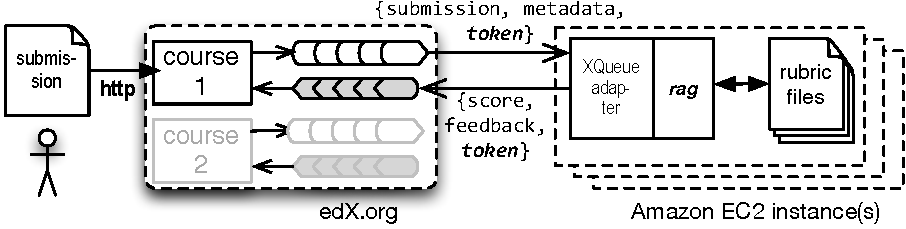
\includegraphics[width=0.75\textwidth]{figs/autograder_arch.pdf}
  \caption{\label{fig:autograder_arch}
  Since our autograders rely on many libraries,
  tools, support files, and so on, we encapsulate the autograder in a
  virtual machine image that is deployed on Amazon Elastic Compute Cloud.
  When a new instance is started, the autograder script automatically runs from
  \texttt{/etc/init.d} and examines a deploy-time environment variable
  to get obtain the credentials needed to make calls to the XQueues.}
\end{figure}


Our initial implementation of autograding was designed to work with
Coursera and later transitioned to OpenEdX.  Both the API and the student
experience are similar 
between the two.  A logged-in student navigates to a page
containing instructions and handouts for a homework assignment;
when ready, the learner submits a single file or a
\texttt{tar} or \texttt{zip} archive through a standard HTTP
file-upload form.  A short time later, typically less than a minute, the
student can refresh the page to see feedback on her work from the
autograder.  

As Figure~\ref{fig:autograder_arch} shows, 
the student's submitted file, plus
submission metadata specified at course authoring time, go into a
persistent queue in the OpenEdX server; each course has its own queue.
We use the metadata field to distinguish different
assignments so that the autograder knows which engine and rubric files
must be used to grade that assignment.
The OpenEdX LMS defines an authenticated RESTful
API\uf{edx-partner-course-staff.readthedocs.org/en/latest/exercises\_tools/external\_graders.html}
by which external standalone autograders can retrieve student
submissions from these queues and later post back a numerical grade and
textual feedback.
The external grader does not have access to the identity of the learner;
instead, an obfuscated token identifies the learner, with the mappings
to the learners' true identities maintained only on OpenEdX.
Hence no sensitive information connecting a work product to a specific
student is leaked if the autograder is compromised.
%% Retrieving an
%% assignment and posting back a 
%% grade are separate queue operations, to allow for autograders that may
%% take a long time to run.  
%% If the autograder polls the XQueue and finds it empty, the grader
%% process sleeps for awhile and tries again.  (In the future we will allow
%% idle autograders to kill themselves.)
Once a submission is retrieved from the queue, the metadata identifies
which grader engine and instructor-supplied rubric files (described
subsequently) should be 
used to grade the assignment.  Finally, a numerical score and 
text feedback from the autograder 
are posted back to OpenEdX.
This simple architecture keeps the grader process stateless, thereby 
simplifying the implementation of cloud-based graders in three ways:

\noindent\textbf{1. No data loss.}
If an assignment is retrieved but no grade is posted back before
a pre-set timeout, OpenEdX eventually returns the ungraded assignment to
the queue, where it will presumably be picked up again by another
autograder instance.
Therefore, if an autograder crashes while grading an assignment, no
student work is lost.

\noindent\textbf{2. Scale-out.} 
Since the autograders are stateless consumers
contacting a single producer (the queue), and grading is
embarrassingly task-parallel, we can drain the queues faster by simply
deploying additional autograder instances.
Since we package the entire autograder and supporting libraries as a
virtual machine image deployed on Amazon's cloud, deploying an
additional grader is essentially a one-click operation. (We have not
yet had the time to automate scaling and provisioning.)
\footnote{OpenEdX also supports an alternative ``push'' protocol in which each student
submission event triggers a call to a RESTful autograder endpoint.
We do not use this
alternative protocol because it thwarts this simple scaling technique
and because we would be  unable to limit the rate at which
submissions were pushed to our autograders during peak times.}
Even our most sophisticated autograders take less than one
machine-minute per assignment, so at less than 10 cents per machine-hour,
MOOC-scale 
autograding is cost-effective and fast: even with
thousands of assignments being submitted in a 50,000-learner course,
students rarely waited more than a few minutes to get feedback.

\noindent\textbf{3. Crash-only~\cite{candea:crash-only}.}
If the external grader crashes (which it does periodically), it can
simply be restarted, which we in fact do in the
body of a \texttt{while(true)} shell script.
If the entire VM becomes unresponsive, for example if it becomes
corrupted by misbehaving student code, it can be rebooted or
undeployed as needed, with no data loss.

In short, the simple external grader architecture of OpenEdX provides a
good separation 
of concerns between the LMS and autograder authors.

\subsection{CI Workflow for Autograders}

Since at any given time the autograders
may be in use by the MOOC and several campus SPOCs, it is important to 
avoid introducing breaking changes to rubric files, homework
assignments, or the autograders themselves.
We set up continuous
integration tasks using Travis-CI, which is integrated with GitHub.
When a pull request is made\footnote{A pull request is
  GitHub's term for the mechanism by which a developer requests that a
  set of changes 
  be merged into the production branch of a codebase.},  
the CI task instantiates  a
new virtual 
machine, installs all the needed software to build an autograder image
based on the codebase as it would appear after the pull request,
and tests the autograder with known solutions versioned with each homework, as
Figure~\ref{fig:rag-ci} shows.
%% These CI features run the autograders locally against
%% inputs via the Open3 library in order to control output streams and
%% return codes. 
Each homework assignment repository also has a CI task that
automates the installation of the autograders and verifies their
configuration. 

%% \begin{figure}[!htbp]
%%   \centering
%%   \begin{minipage}{0.70\textwidth}%
%%   \lstset{tabsize=1,basicstyle=\scriptsize\ttfamily}%
%%   \lstinputlisting{figs/travis.yml}%
%%   \end{minipage}
%%   \caption{\label{fig:rag-ci}%
%%   Typical .travis.yml file.
%% }
%% \end{figure}

\begin{figure}
  \centering
  \lstinputlisting[tabsize=1,basicstyle=\scriptsize\ttfamily]{figs/ci_feature.txt}%
  \lstinputlisting[tabsize=1,language=Ruby,basicstyle=\scriptsize\ttfamily]{figs/ci_stepdefs.rb}%
  \caption{\label{fig:rag-ci}%
  Top: Cucumber integration test that is run whenever the autograder or
  homework code is updated.  (Cucumber is described in the next
  section.)
  The scenarios verify that, at a minimum,
  the autograder reports a score of 100\% when run against the
  instructor's reference solution and a score of 0\% when run against
  the empty ``code skeleton'' provided to students.  
  Bottom: examples of the Cucumber step definitions invoked when these
  steps are run.
}
\end{figure}


\section{\emph{rag}, a Ruby Autograder for ESaaS}

Having chosen Ruby and Rails for their excellent testing and
code-grooming tools, our approach was to repurpose those same tools into
autograders that would give finer-grained feedback than human graders
using more detailed tests, and would be easier to repurpose than
those built for other languages.

\begin{figure}
  \begin{tabular}{|p{0.15\textwidth}|p{0.15\textwidth}|p{0.7\textwidth}|}
 \hline
 \textbf{Grader} & \textbf{Based on} & \textbf{Student Assignment Type} \\
 \hline
 RSpecGrader &
 unit testing &
 Student submits one or more class files; black-box and ``intrusive''
 unit tests against functions and groups of functions are performed
 \\
 FeatureGrader &
 simplified mutation testing &
 Student submits integration tests written using Cucumber; bugs inserted
 in reference app attempt to trigger test failures to check test suite
 completeness and test fragility
 \\
 MechanizeGrader & 
 staging-like integration testing &
 Student deploys full-stack app to public cloud; ``black box'' tests
 stimulate remote server and parse/analyze output, including execution
 of JavaScript if needed
 \\
 \hline
\end{tabular}

  \caption{\label{fig:grader_summary} Summary of the autograder
    engines based on our repurposing of excellent existing open-source
    tools and testing techniques.  Only the RSpecGrader is
    Ruby-specific; the others are easily retargetable to other languages
    and systems.}
\end{figure}

\texttt{rag}\uf{github.com/saasbook/rag} 
is actually a collection of three different autograding
``engines'' based on open-source testing
tools, as Figure~\ref{fig:grader_summary} shows.  
Each engine takes as input a student-submitted work
product and one or more rubric files, and grades the work according to
the rubric.  The contents of the rubric files depend on the type of
engine used.\footnote{Currently the rubric files must be present in the
  local filesystem of the autograder VM, but refactoring is in progress
  to allow these files to be securely loaded on-demand from a remote
  host so that currently-running 
  autograder VMs do not have to be modified when an assignment is added
  or changed.}
The first of these is
\textbf{RSpecGrader}, based on RSpec, an XUnit-like 
TDD framework that exploits Ruby's
flexible syntax to embed a highly readable unit-testing DSL in Ruby.
The instructor annotates specific tests within an assignment with point
values (out of 100 total); RSpecGrader computes the total points
achieved and concatenates and formats the error/failure messages from
any failed tests, as Figure~\ref{fig:rspec_grader_rubric} shows.
RSpecGrader  runs RSpec in a separate timer-protected interpreter
thread in which large sections of the
standard library such as file I/O and most system calls have been
stubbed out, allowing us to handle exceptions in RSpec itself as well
as test failures.  

\begin{figure}
  \centering
    \lstinputlisting[numbers=left,tabsize=1,basicstyle=\scriptsize\ttfamily]{figs/rspec_grader_rubric.rb}
  \caption{\label{fig:rspec_grader_rubric}
    In an RSpecGrader rubric, some test cases are ``sanity checks''
    without which the assignment isn't even graded
    (lines 2--9) while others contribute points to the
    student's score.  Ruby's dynamic language features allow us to
    easily check, for example, that
a student's implementation of a ``sum all the numbers'' method does not
simply call a built-in library method (line 7).
  }
\end{figure}

A variant of RSpecGrader is \textbf{MechanizeGrader}.
Surveys of recent
autograders~\cite{ihantola-2010-autograding-survey,douce-2005-autograding-survey}
mentioned as a ``future direction'' a grader that can assess full-stack
GUI applications.
MechanizeGrader does this using Capybara and
Mechanize\footnote{\url{jnicklas.github.io/capybara},
\url{rubygems.org/gem/mechanize}}.
Capybara provides a Ruby-embedded DSL for interacting with Web-based
applications by providing primitives that trigger actions on a web page
such as filling in form fields or clicking a button, and examining the
server's delivered results pages using XPath\uf{w3.org/TR/xpath20/}, as
Figure~\ref{fig:mechanize_grader_example} shows. 
Capybara is usually used as an in-process testing tool, but Mechanize
can trigger Capybara's actions against a remote application, allowing
black-box testing.
Students' ``submission'' to MechanizeGrader is therefore the URL to their
application deployed on the public 
cloud.  (We use the free tier of Heroku for our assignments and
projects.)

\begin{figure}
 \centering
  \lstinputlisting[language=Ruby,numbers=left]{figs/mechanize_grader_example.rb}
  \caption{\label{fig:mechanize_grader_example} 
This excerpt of three test cases from a MechanizeGrader rubric runs
against a student's 
deployed full-stack application.}
\end{figure}

Finally, one of our assignments requires students to write integration-level
tests using Cucumber, which allows such tests to be formulated in
stylized plain text, as Figure~\ref{fig:cucumber} shows.
Our autograder for this
style of assignment is inspired by mutation testing, a technique invented
by George Amman and Jeff 
Offutt~\cite{ammann-offutt-sw-testing} in which a
testing tool pseudo-randomly mutates the program under test to ensure
that some test fails as a result of these introduced errors.

\begin{figure}
  \centering
    \lstinputlisting{figs/cucumber_example.feature}
    \lstinputlisting[language=Ruby]{figs/cucumber_step_def_example.rb}%
  \caption{\label{fig:cucumber} Cucumber accepts integration tests 
    written in stylized prose (top) and uses regular expressions to map each
    step to a \emph{step definition} (bottom) that sets up preconditions, exercises the app,
    or checks postconditions.  Step definitions 
    can stimulate a full-stack GUI-based web application in various
    ways, including remote-controlling a real browser with Webdriver
    (formerly Selenium) or using the Ruby Mechanize library to interact
    with a remote site.  Our code blocks are in Ruby, but the Cucumber framework
itself is polyglot.} 
\end{figure}

Specifically, \textbf{FeatureGrader} operates by working with an
existing application to which student-created tests will be applied.   The application is modified so that the FeatureGrader
can adjust the application's behavior by manipulating certain environment variables. Each  scenario 
specified by the assignment is first tested against the working application.  Assuming the 
students have created the correct acceptance tests in Cucumber, all these tests should pass.  

Next the FeatureGrader starts to mutate the underlying application
according to a simple specification (Figure~\ref{fig:featuregrader}), running the specified feature against
the mutated application and checking that the specified scenarios do in fact fail.  Students 
lose points according to the weights associated with features that do not generate the expected failure.


\begin{figure}
  \begin{minipage}{0.45\textwidth}%
  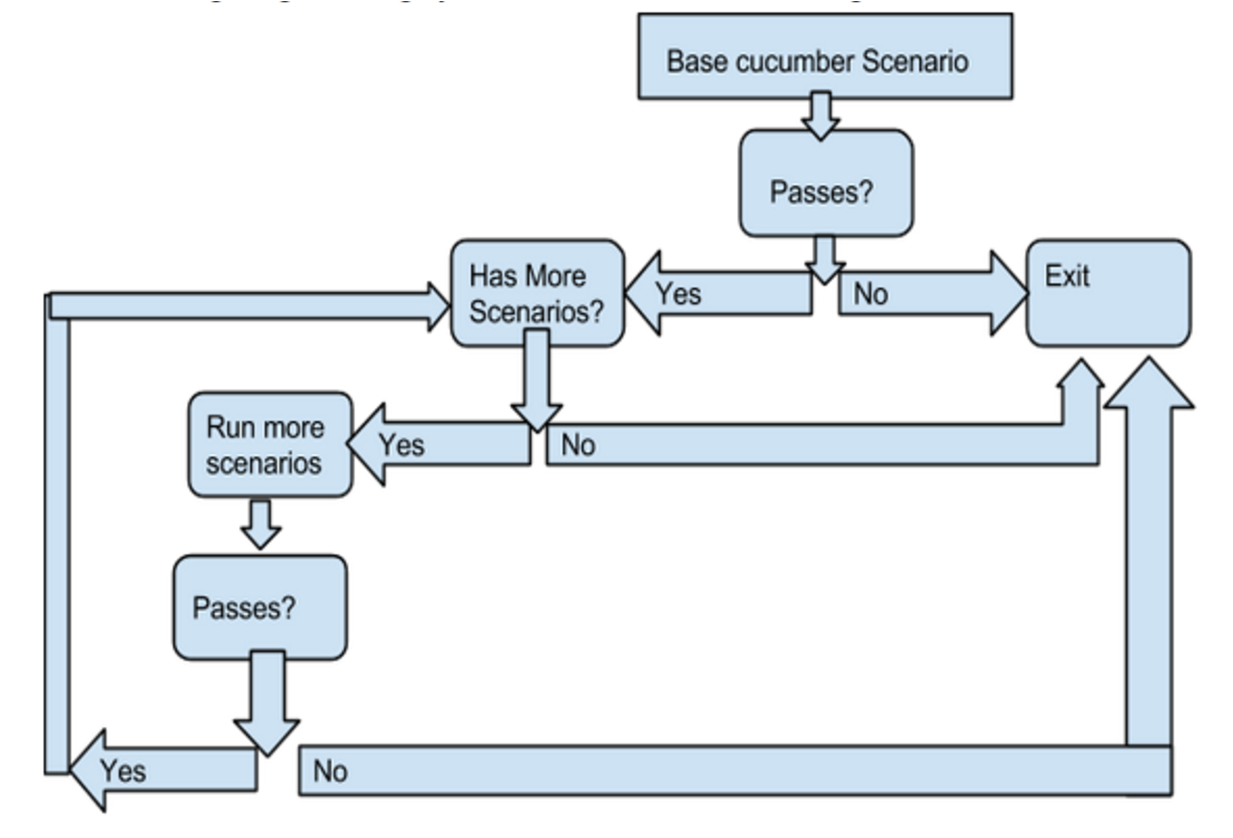
\includegraphics[width=\textwidth]{figs/feature_grader.pdf}%
  \end{minipage}%
  \begin{minipage}{0.55\textwidth}%
  \lstinputlisting{figs/feature_grader_example.yml}%
  \end{minipage}
  \caption{\label{fig:featuregrader}%
FeatureGrader workflow and example YAML file.  In this case if Step1-1 passes,
Step1-3 will be run next.  Earlier steps must be less restrictive than
later steps (if the earlier step fails, there should be no way that a later one could pass).
\texttt{failures} are the two student-provided Cucumber scenarios that \emph{should fail} when
run because of mutations (bugs) inserted in the app.
}
\end{figure}


\section{Discussion}



a.	Value of tools ecosystem in Rails world. Majority of new autograders in 2010 survey were either for Java or language-neutral with output checking only. We had good reasons for using Ruby and still do. Student feedback in campus course bears this out.


When we set about revising the Software Engineering course in which
these autograders are used, our choice of Ruby and Rails was not without
controversy.  Some students complained about having to learn another
language (the three lower-division courses that form the gateway into
the major are taught in Python, Java, and C), despite our assurances
that they would need this skill  as professional developers, learning a
new language every three or four years.  Our view was, and continues to
be, that the superior tools for testing, code analysis and code grooming
available in Ruby resulted in higher productivity and student engagement
that justified this learning curve.  What we did not anticipate was that
we ourselves would ultimately turn to these same tools to facilitate
automated grading.  Of the three autograders we have described, only the
RSpecGrader is Ruby-specific.



b.	Getting unnecessary stuff out of the way: avoid wasting student time with admin, setup, etc.  

1.	VM provides courseware; maybe soon C9.  

2.	Heroku provides deployment.  

3.	OpenEdX presents the HW explanations, videos, selfcheck questions along the way using RuQL (cite), inspired by ideas like OKgrader (cite)

c.	Challenge: tuning rubrics. Use campus course to debug.

Challenge: avoding "autograder-driven development"


d.	Challenge: stability. By and large edX works.  Good separation
of concerns between LMS and autograder authors.

e.	Challenge: test suite quality. THis si a general problem in SWE. Example: if multiple tests are effectively redundant, student scoring is positively distorted if all pass and negatively distorted if all fail.




\section{Conclusions}



a.	Both surveys ask why existing autograders aren't reused more.

b.	SPOC instructors using it as part of overall ESaaS; hosted on edge.edx.org through arrangement with me; advise Sam interested

c.	Can also stand up your own OpenEdX and use our graders as a service. Contact Sam.

d.	Or take the code and create another adapter for it to plug into your favorite campus system (we'd love an LTI adapter).  Github pointer.




\subsubsection*{Acknowledgments}  % don't change the section header type!

We thank  Google for early support of this effort as well as support
for the current refactoring to further scale the courses that use this
technology. 
We thank the technical teams at Coursera and edX for their  early
support for this course by providing the necessary external grader APIs.
We thank the AgileVentures team for both helping steward the MOOC and
providing substantial development and maintenance effort on the
autograders, especially with their contribution of the CI workflows.

Finally, thanks to the many, many UC~Berkeley undergraduate and graduate
students who have contributed to the development of the autograders,
including
James Eady, 
David Eliahu, 
Jonathan Ko, 
Robert Marks,
Mike Smith,
Omer Spillinger,
Richard Xia, 
and
Aaron Zhang.


\bibliographystyle{splncs03}
\bibliography{magic}

\end{document}
